\documentclass[../main.tex]{subfiles}

% ======================== Document: Results ======================== %

\begin{document}
\section{Results}
\label{sec:results}

\subsection{Patent applications}

Table \ref{tab:dd_twfe_patents} presents results the estimation of Equation \ref{eq:dd_model} using patent applications as the explained variable with the province-quarter data. Specification (1) includes a baseline result with no control variables. Specification (2) includes economic controls included to account for factors which may affect the comparability of the treatment and control groups regarding firm activity and overall economic trends which vary across time and provinces. The number of foreign parties in all the province's patent applications is also included, to control for effects that foreign interested parties (particularly U.S.) can have as strategic actors for patent applications. Specification (3) considers additional controls, which are included in case that the previous ones did not account for differences in trends due to reasons other than economy, or that economic activity is not well captured by standard economic variables in Specification (2). 

The DD estimate for the effect of the AITC intervention is the coefficient on Treatment \texttimes Post, showing that the intervention led to an -6.1\% to +2.3\% change in Albertan patent applications. The baseline specification shows a negative effect, while the other two specifications show positive effects. However, these are not statistically distinguishable from zero. Standard errors for this coefficient on all three specifications are small compared to those of the controls, showing that $\hat{\beta}$ is estimated with a fairly good level of precision. This implies that it is the small magnitude of $\hat{\beta}$ which drives the low $p$-value of the hypothesis test, leading to the preliminary conclusion that the AITC intervention had no effect on innovation in the studied period. 

\begin{table}[htbp!]
    \centering
\begin{threeparttable}
    \caption{Difference-in-differences specifications for quarterly patent applications}
    \label{tab:dd_twfe_patents}
    
\begin{tabular}[t]{lccc}
\toprule
  & (1) & (2) & (3)\\
\midrule
Treatment x Post & \num{-0.093}* & \num{0.001} & \num{-0.011}\\
\textbf{} & \textbf{(\num{0.042})} & \textbf{(\num{0.066})} & \textbf{(\num{0.076})}\\
Ln Full-time employment &  & \num{0.756} & \num{1.032}\\
 &  & (\num{0.644}) & (\num{0.646})\\
Ln Median wage &  & \num{1.235}** & \num{1.107}**\\
 &  & (\num{0.387}) & (\num{0.445})\\
CPI &  & \num{-0.015}** & \num{-0.007}\\
 &  & (\num{0.005}) & (\num{0.008})\\
Ln +1 Business insolvencies &  & \num{-0.065}** & \num{-0.051}*\\
 &  & (\num{0.027}) & (\num{0.023})\\
Ln Intl. exports &  & \num{-0.081} & \num{-0.079}\\
 &  & (\num{0.097}) & (\num{0.125})\\
Ln Intl. imports &  & \num{0.016} & \num{0.022}\\
 &  & (\num{0.126}) & (\num{0.127})\\
Ln Retail sales &  & \num{-0.279} & \num{0.094}\\
 &  & (\num{0.421}) & (\num{0.492})\\
Ln Wholesale sales &  & \num{-0.150} & \num{-0.229}\\
 &  & (\num{0.156}) & (\num{0.139})\\
Ln Manufacturing sales &  & \num{0.275} & \num{0.210}\\
 &  & (\num{0.153}) & (\num{0.146})\\
Ln +1 Foreign patent parties &  & \num{0.141}*** & \num{0.135}***\\
 &  & (\num{0.016}) & (\num{0.016})\\
Ln International travellers &  &  & \num{-0.129}***\\
 &  &  & (\num{0.034})\\
Ln Arriving vehicles &  &  & \num{0.007}\\
 &  &  & (\num{0.004})\\
Ln Electric power generation &  &  & \num{0.078}\\
 &  &  & (\num{0.115})\\
Ln Average actual hours &  &  & \num{0.109}\\
 &  &  & (\num{0.277})\\
New housing price index &  &  & \num{-0.003}\\
 &  &  & (\num{0.002})\\
Ln Food services receipts &  &  & \num{-0.080}\\
 &  &  & (\num{0.201})\\
Ln Average job tenure &  &  & \num{-0.424}\\
 &  &  & (\num{0.373})\\
\midrule
Explained variable &  & $\ln(\text{Patents}+1)$ & \\
$N$ & \num{656} & \num{656} & \num{656}\\
Adj. $R^2$ & \num{0.975} & \num{0.980} & \num{0.980}\\
Adj. within $R^2$ & \num{0.002} & \num{0.205} & \num{0.210}\\
RMSE & \num{0.206} & \num{0.182} & \num{0.180}\\
\bottomrule
\end{tabular}
}
    \begin{tablenotes}
        \small
        \item \textit{Notes}: Clustered standard errors at the province and quarter level shown in parentheses. All specifications include fixed effects for provinces and quarters. ***$p<0.01$, **$p<0.05$, *$p<0.1$.
    \end{tablenotes}
\end{threeparttable}
\end{table}

I display the results of the event study regressions in Figure \ref{fig:event_study_patents}. I estimated Equation \ref{eq:event_study} with the same controls as the specifications in Table \ref{tab:dd_twfe_patents}, resulting in panels (1) through (3) plotted in Figure \ref{fig:event_study_patents}. Most importantly, these results show that when controlling for time and province-varying factors, there is not a statistically significant difference between Albertan and control provinces patent applications before the intervention. This supports the key identifying assumption of the DD design. The baseline model shows several pre-policy periods where the treatment and control groups diverge, underscoring the importance of including controls in the model. However, in all specifications 2015Q4 presents a statistically significant difference in patent applications between the treatment and control groups. This can be due to random noise or to a temporary real effect, however, since it is only one period which is significant, it does not greatly threaten causal identification of the AITC effect. 

\begin{figure}[htbp!]
    \centering
    \caption{Event study plot for quarterly patent applications}
    \label{fig:event_study_patents}
    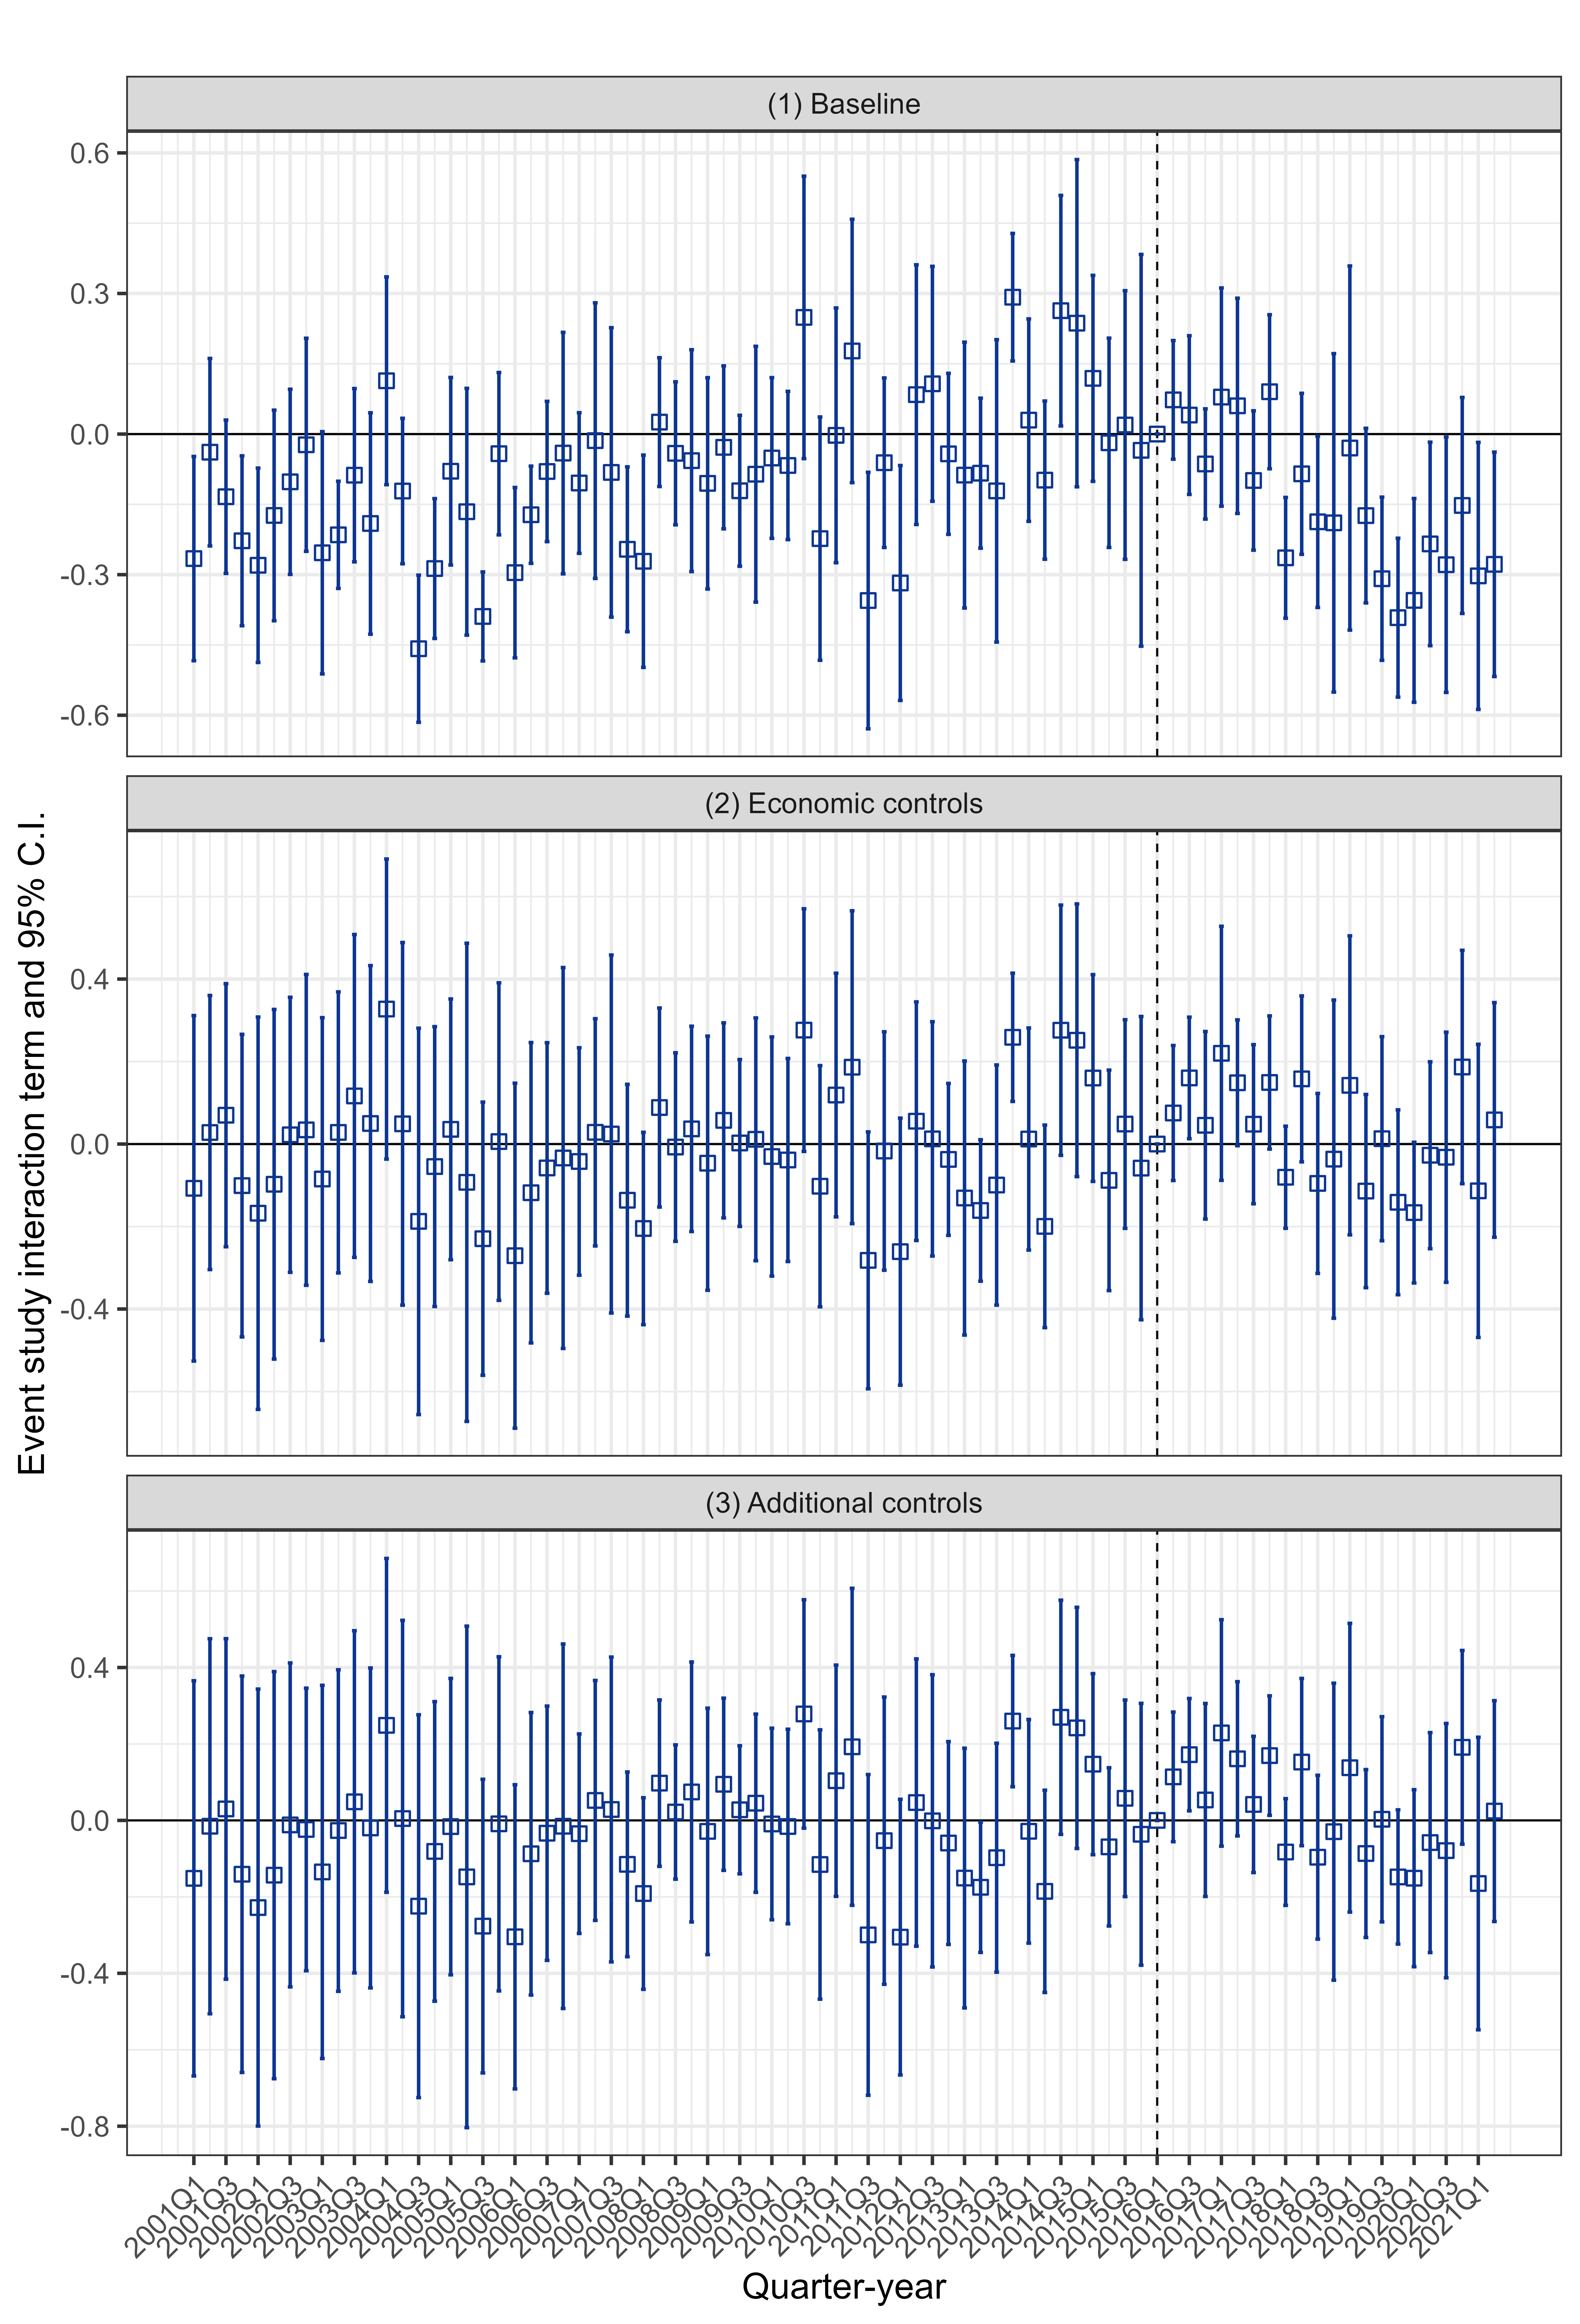
\includegraphics{\subfix{../../figures/event-studies/quarterly/patents_faceted.png}}
    \begin{minipage}{0.9\textwidth}
        \footnotesize
        \textit{Notes}: The figure shows the estimated coefficients of the interaction term between period and treatment binary variables in Equation \ref{eq:event_study} for each quarter. The points represent the point estimate, while the error bars represent the 95\% confidence cluster-robust interval. The vertical line represents the start of the AITC intervention (first expense eligibility date) in April 2016, with the reference level being the quarter before the intervention. Baseline, economic, and additional controls specifications include the controls seen in specifications (1) through (3) in Table \ref{tab:dd_twfe_patents}. 
    \end{minipage}
\end{figure}

% Note: need to add a row with the number of identified patent applications to make the table more informative.

Regarding the effect of the policy itself, results point toward an overall null effect. While there is a small positive effect in 2016Q4, it is unlikely that this is due to the policy, as the effect is not present in the following quarters. There is also no evidence of a negative effect of the policy on patent applications, as preliminarily shown by the time series plot in Figure \ref{fig:quarterly_common_trends}.

\subsection{Patents by IPC section}

In Table \ref{tab:dd_twfe_patents_by_section}, I present the results of the estimation of Equation \ref{eq:dd_model}, allowing for heterogeneity by IPC patent section and including the controls of Specification (3) in Table \ref{tab:dd_twfe_patents}. The results show that the AITC intervention had no statistically significant effect on most of the IPC sections, except sections A and E, corresponding to human necessities and fixed constructions. The effect on section A is positive and significant, while the effect on section E is negative and significant. These two effects are of similar magnitude (between 42.7\% to 53.0\% in absolute value), suggesting an offseting effect of the policy. 
   
\begin{table}[htbp!]
    \centering
\begin{threeparttable}
    \label{tab:dd_twfe_patents_by_section}
    \caption{Difference-in-differences results for quarterly patent applications by IPC section}
    
\begin{tabular}[t]{lcccccccc}
\toprule
  & (1) & (2) & (3) & (4) & (5) & (6) & (7) & (8)\\
\midrule
Treatment x Post & \num{0.427}*** & \num{0.366} & \num{0.066} & \num{0.235} & \num{-0.530}*** & \num{0.167} & \num{-0.083} & \num{0.209}\\
\textbf{} & \textbf{(\num{0.071})} & \textbf{(\num{0.195})} & \textbf{(\num{0.171})} & \textbf{(\num{0.132})} & \textbf{(\num{0.045})} & \textbf{(\num{0.106})} & \textbf{(\num{0.187})} & \textbf{(\num{0.135})}\\
\midrule
Patent section (IPC) & A & B & C & D & E & F & G & H\\
$N$ & \num{656} & \num{656} & \num{656} & \num{656} & \num{656} & \num{656} & \num{656} & \num{656}\\
Adj. $R^2$ & \num{0.913} & \num{0.911} & \num{0.879} & \num{0.353} & \num{0.914} & \num{0.875} & \num{0.910} & \num{0.908}\\
Adj. within $R^2$ & \num{0.111} & \num{0.056} & \num{0.082} & \num{0.033} & \num{0.061} & \num{0.021} & \num{0.060} & \num{0.063}\\
RMSE & \num{0.324} & \num{0.355} & \num{0.381} & \num{0.356} & \num{0.361} & \num{0.394} & \num{0.395} & \num{0.409}\\
\bottomrule
\end{tabular}
}
    \begin{tablenotes}
        \footnotesize
        \item \textit{Notes}: Sections of the IPC are A: Human Necessities, B: Performing Operations; Transporting, C: Chemistry; Metallurgy, D: Textiles; Paper, E: Fixed Constructions, F: Mechanical Engineering; G: Physics, H: Electricity. Patents with multiple sections are not included. All specifications include controls in Specification (3) of Table \ref{tab:dd_twfe_patents}, not shown for brevity and fixed effects for provinces and quarters. Clustered standard errors at the province and quarter level shown in parentheses. ***$p<0.01$, **$p<0.05$, *$p<0.1$.
    \end{tablenotes}
\end{threeparttable}
\end{table}

% Note: need a row with the number of identified patent applications by section to make the table more informative.
% Should also try to make the table less wide so that it fits within the page.

Given that there is a smaller number of patents per IPC section for all provinces, I am underpowered to detect small effects on the other sections which presented null effects. The event study regressions in Figure \ref{fig:event_study_patents_section} provide additional insight about the intervention's effect on patent applications by IPC section. The figure displays the same coefficients and confidence intervals as those of in Figure \ref{fig:event_study_patents} separating by IPC section and restricting to the additional controls specification. 

\begin{figure}[htbp!]
    \centering
    \caption{Event study plot for quarterly patent applications by IPC section}
    \label{fig:event_study_patents_section}
    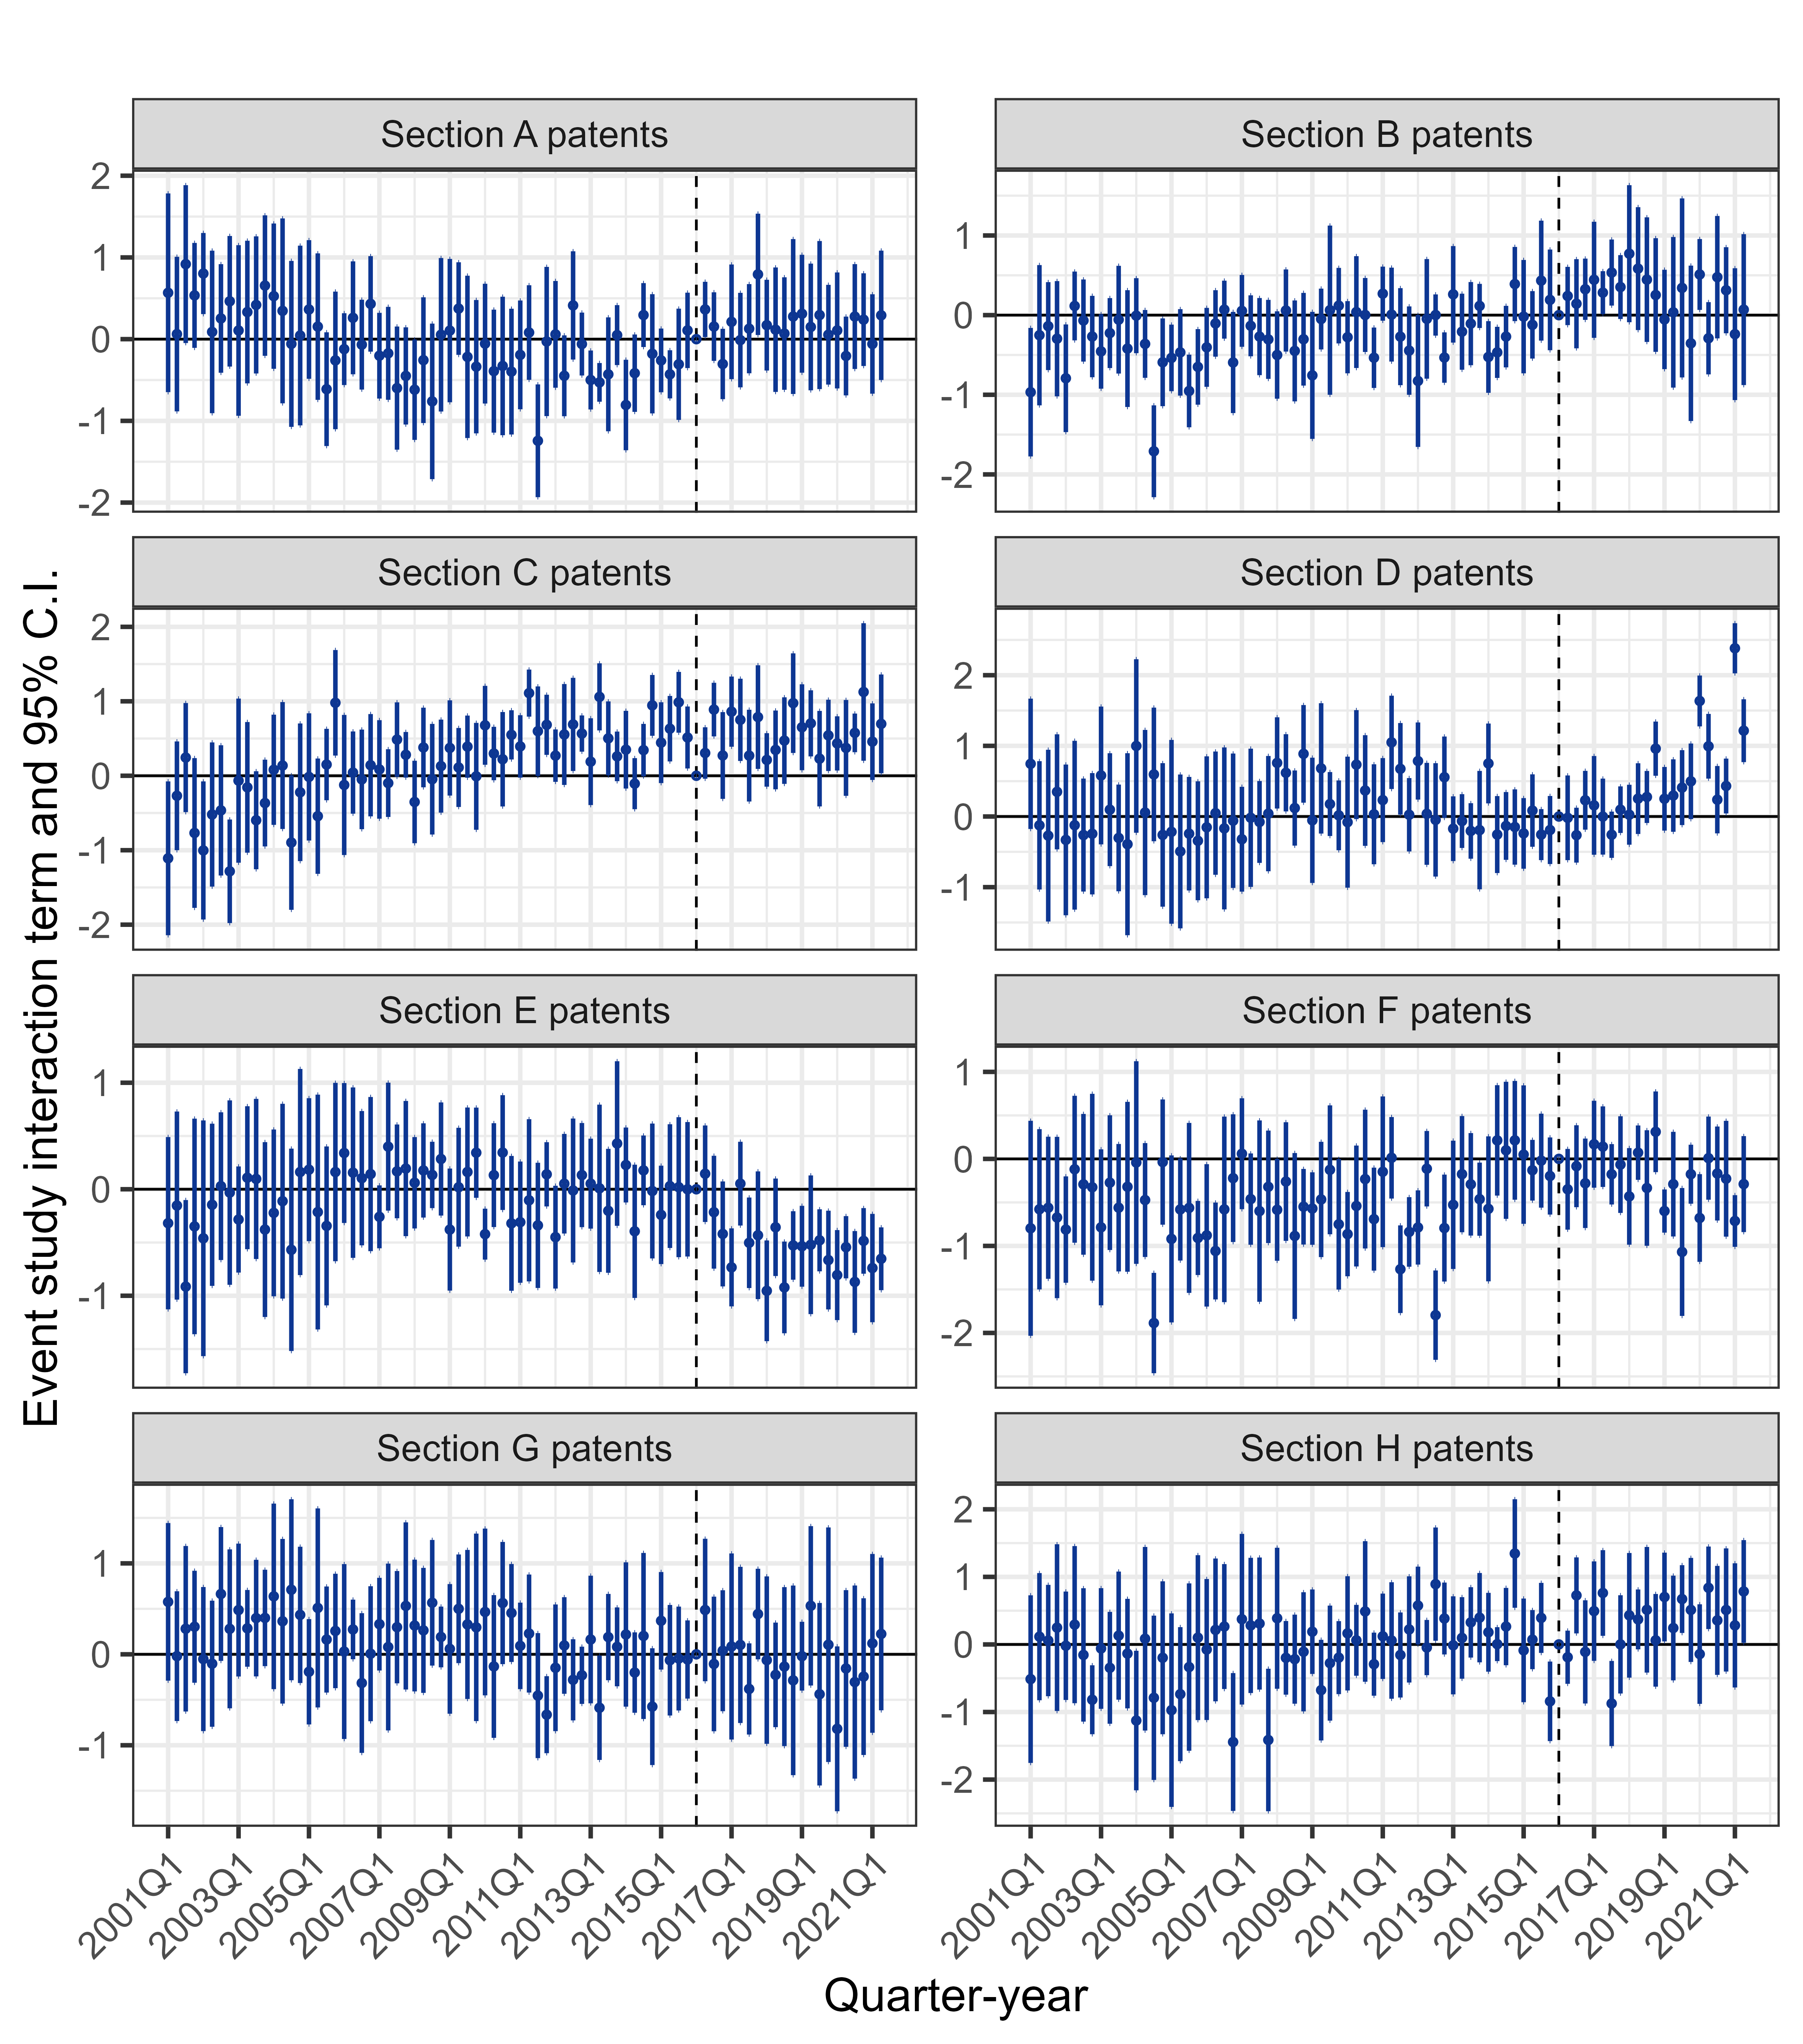
\includegraphics{\subfix{../../figures/event-studies/quarterly/patent_sections_faceted.png}}
    \begin{minipage}{0.9\textwidth}
        \footnotesize
        \textit{Notes}: The figure shows the estimated coefficients of the interaction term between period and treatment binary variables in Equation \ref{eq:event_study} for each quarter, separating by IPC section. The points represent the point estimate, while the error bars represent the 95\% confidence cluster-robust interval. The vertical line represents the start of the AITC intervention (first expense eligibility date) in April 2016, with the reference level being the quarter before the intervention. Controls are the same as those in Specification (3) in Table \ref{tab:dd_twfe_patents}. 
    \end{minipage}
\end{figure}

% need to include definition of human necessity

Human neccessity (A) patents, which include agriculture, medicine and apparel related inventions, show only one significant deviation from the pre-policy trend, five quarters after the intervention (2017Q3). These patents increased by approximately 79\% relative to one period before the intervention. However pre-intervention coefficients are less stable for this section, potentially due to its broad definition.

Fixed constructions (E) patents, which include patents related to buildings, roads, and bridges, do show a significant decrease in most quarters after the intervention. Pre-policy coefficients are stable, and the effect is present in the first quarter after the intervention, suggesting that the policy may have had a negative effect on this type of patent applications. Because the policy did not particularly target this type of innovation, it is possible that this type of innovation may have been crowded out by other types of inventions. 

Other notable results which were not picked up by the DD specification are in the Section D patents, which include patents related to textiles and paper. While less stable than other sections, these patents show the most important increase of all patent sections, the highest increase being 238\% more patent applications 19 quarters after the intervention (Q32020). The pre-policy trend is mostly common across the treatment and control groups (with the exception of 2015Q4, same as in the total patent event study), suggesting that these increases were due to the AITC intervention. The DD may not capture this effect due to increases being present next to quarters without increases. 

% change methods to include ipc sections as part of the analysis
% including monthly analysis is part of robustness checks
% including patent parties is a robustness check

\subsection{Robustness checks}



\end{document}